\chapter{Probabilistic model}\label{chap:prob_model}
Since the proposed approach implements a probabilistic validation, the reliability of the validation depends on the number of validators in the network in relation to the size of input. Given that the number of validators is finite, the probability of accepting an invalid result may exceed an acceptable threshold for big inputs. Thus, the distributed assertion checking scheme should provide a mechanism to have each validator invoke the assertion contract a specified number of times. To this end, it is necessary to identify a formula which, given the input size and a probability threshold, returns a lower bound for the required number of test runs per validator. 

Sections \ref{sec:coupon} and \ref{sec:prob_threshold} describe the findings from a collaborative work with Julian Veigl \cite{bernhardt_veigel_2020}. They are based on the assumption that random generators pick elements independently from a uniform distribution. Furthermore, all calculations are based on the worst case scenario, in which there exists exactly one counterexample for the validity of the given input.

\section{Sample spaces}
The sample space of an assertion is given by the domains of discourse of the quantifiers. \secref{sec:transf_domains} described, that the premises defining the domains are translated into a list of range constraints for the random generators. Based on these constraints, the compiler can derive a formula to determine the size of the sample space at runtime. In simple cases, the sample space is given by a single domain. Such a space is given, for instance, in the introductory example checking whether a number is a prime, i.e., $\mathcal{S} = \lbrace n \in\mathbb{Z} : 2 \le n \le \sqrt{p} \rbrace$. Based on the constraints $2 \le n$ and $n \le \sqrt{p}$, the size of the search space can be determined at runtime with $|\mathcal{S}| = \sqrt{p} - 2$. If the assertion has to sample from more than one domain, the search space is given by the Cartesian product of these domains. In the example of intersecting sets from \secref{sec:existential}, the sample space is $\mathcal{S} = \mathcal{S}_U \times \mathcal{S}_V$, where $\mathcal{S}_U = \lbrace n \in\mathbb{Z} : 0 \leq n \le |U| \rbrace$ and $\mathcal{S}_V = \lbrace m \in\mathbb{Z} : 0 \leq m \le |V| \rbrace$). At runtime, the size of the search space can be determined with $|\mathcal{S}| = (|U| - 0) + (|V| - 0)$.

\section{Coupon Collector's Problem Analysis}\label{sec:coupon}
When checking properties with probabilistic testing, the result is either definitely not satisfied, or probably satisfied. Thus, errors only occur as false positives. In order to find a counterexample with probability $p = 1$, every element in the given search space $\mathcal{S}$ has to be checked by at least one validator. Deterministically, this is reachable with exactly $|\mathcal{S}|$ test runs. This is, however, invalid for the probabilistic approach, as some validators may generate the same random values and thus leave some elements of $\mathcal{S}$ unchecked. \\
In probability theory, this is known as the Coupon Collector's Problem \cite{croucher_collecting_2006}. Given $n = |\mathcal{S}|$, the probability that $n$ validators generate a unique element from $\mathcal{S}$ is given by
\begin{equation*}
    p = \prod_{i=1}^{n} \frac{i}{n}
\end{equation*}
As an example, the probability already drops to $0.036\%$ for $n = 10$.

Let the random variable $T$ be the number of completed test runs until every element in the search space has been generated at least once. By identifying its expectation $E(T)$, one can obtain an estimation of how many test runs are needed to find the counterexample with certainty. Since a generated value can either be unique (``success'') or a duplicate (``failure''), a test run can be seen as a Bernoulli trial \cite{papoulis02}. Therefore, the geometric probability distribution is applied \cite{croucher_collecting_2006}.

Each element is generated with a probability of $1/n$. Thus, the probability to generate the $i$th unique element is given by 
\begin{equation}
    p_i = \frac{n-i+1}{n}
\end{equation}
The expected value of a random variable $X$ is given by $E(X) = \frac{1}{p}$, thus the expected number of test runs for $n$ is 
\begin{equation}
E(T) = n \sum_{i=1}^{n} \frac{1}{i}
\end{equation}
\tabref{tab:prob_outcomes} shows the expected number of test runs $E(T)$ and its standard deviation $\sigma$ for different $n$. Furthermore, $E(T)$ and $\sigma$ are used to calculate a 95\% confidence interval for $T$ by applying the central limit theorem, which provides an upper and lower bound on the number of test runs. Rounded values for both bounds are also shown in \tabref{tab:prob_outcomes}.
\begin{table}[h]
    \centering
    \begin{tabular}{lllll}
        \thead{$n$} & \thead{$E(T)$} & \thead{$\sigma$} & \thead{lower bound} & \thead{upper bound}\\ \hline
        5 & 11.4 & 2.53 & 6 & 16\\
        10 & 29.3 & 4.32 & 21 & 38\\
        20 & 72.0 & 7.21 & 58 & 86\\
        30 & 119.8 & 9.48 & 101 & 138 \\
        50 & 225.0 & 13.23 & 199 & 251 
    \end{tabular}
    \caption{Expectation, standard deviation and upper and lower bound of needed test runs for some $n$ \cite{croucher_collecting_2006}}
    \label{tab:prob_outcomes}
\end{table}

The results show that checking random values is a very inefficient approach if false positives are not admissible and an error rate of close to zero is targeted. Even if the lower bound of $T$ is chosen as the number of test runs, it exceeds the size of the search space by far and increases the time complexity to $\mathcal{O}(n*log(n))$ for large $n$ \cite{xu_tang_2011}. For instances where false positives are tolerable, the following section introduces a formula to determine the number of needed test runs to detect counterexamples with a configurable probability.

\section{Configuration of the error rate}\label{sec:prob_threshold}
The goal is to find a number $t$ of test runs, s.t. the probability $P_{c,t}$ of accepting an invalid result falls below a certain threshold $c$. A validator finds the counterexample in one test run with probability $\frac{1}{n}$, and misses it with probability $(1-\frac{1}{n})$. After $t$ tests runs, the probability that the counterexample has not been found is thus $(1-\frac{1}{n})^t$. Following the same approach as Mahlmann and Schindelhauer \cite{mahl_schindel_2007} to retrieve an upper bound for $P_{c,t}$, the following inequality is used:
\begin{equation}
(1-\frac{1}{m})^m \leq \frac{1}{e}
\end{equation}
which holds for all $m > 0$. From this inequality, it follows that
\begin{equation}
(1-\frac{1}{n})^t = ((1-\frac{1}{n})^n)^{\frac{t}{n}} \le e^{-\frac{t}{n}}
\end{equation}
With this, the probability $P_{c,t}$ of missing the counterexample with $t$ test runs can be defined as
\begin{equation}
P_{c,t} \le e^{-\frac{t}{n}}
\end{equation}
In order to determine a value for $t$, s.t. $P_{c,t}$ falls below a specified threshold $c$, the inequality is solved for $t$. The resulting inequality then depends on the known parameter $n$ and an arbitrary value for $c$:
\begin{align}
    e^{-\frac{t}{n}} &\leq c && \text{with } 0 \leq c\le 1 \nonumber\\
    t &\geq -n\:\ln(c)
\end{align}
For $c = \frac{1}{e}$ ($\approx 36.79\:\%$) the lower bound of $t$ is exactly $n$. For lower error rates, the number of test runs needs to be greater than $n$. \figref{fig:graph_t_c} shows the lower bounds of $t$ as a function of the probability threshold and the size of the search space. One can see that the increase of test runs is approximately linear for higher thresholds, but transitions to an exponential testing effort to reach lower thresholds.
\begin{figure}[h]
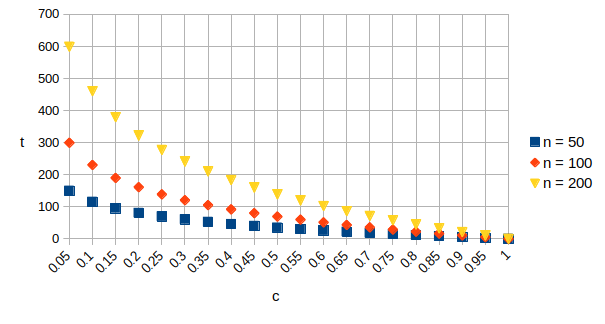
\includegraphics[width=0.95\linewidth]{figures/4-probabilistic_model/graph_t_c}
\caption{Number of required test runs as a function of the probability of false positives $c$ and size of the search space $n$}
\label{fig:graph_t_c}
\end{figure}

\section{Validators vs. test runs}
The last section derived a formula which determines the lower bound of test runs to obtain a specified error rate. However, $t$ is not a parameter that can be adjusted to an arbitrary value on the blockchain. Assuming a blockchain has $m$ validators, the lowest possible bound of test runs is $m$, as every validator invokes the assertion at least once. In cases where $m$ test runs are not sufficient to fall below the threshold $c$, each validator has to invoke the assertion multiple times. More specifically, the number of test runs per validator is given by \eqref{eq:t_validator} and is always a multiple of $m$.
\begin{equation}\label{eq:t_validator}
t_{validator} = \lceil t / m \rceil
\end{equation}

\section{Alternatives to random testing}\label{sec:alt_random}
For applications where low error rates are crucial and random sampling generates too much cost, an alternative could be to coordinate a systematic iteration of the domain. However, the implementation of such a coordination is not trivial, as the validators are engaged via a broadcast and cannot be passed an individual value as input. Instead, possible approaches could be to implement a central instance that allocates an element in the search space to each validator, or to use some unique and intrinsic attribute of validators as a seed or input of a mapping to elements in the search space.

\subsection{Central allocation of elements}
For this approach, the toolchain would need to generate a separate contract that is called by the miners and validators as a proxy. When invoked, this proxy contract allocates the next element of the search space (for instance using a modulo-n counter) and passes this number as an additional parameter to the assertion contract. Furthermore, the proxy contract needs to avoid race conditions in case the assertion mechanism is triggered by several external transactions simultaneously. Another drawback of the proxy contract having to update its internal storage is the consequential serialization of the tests runs.

\subsection{Using unique attributes of a validator}\label{sec:alt_attributes}
This approach strongly depends on whether the validators have a unique id or another attribute, which can be accessed from within a contract. If there is (or the language can be extended with such a feature), the assertion contract needs to implement a non-injective surjective function $f: X_{:A} \rightarrow Y_{:B}$ mapping the respective attribute, represented by a type A, to an element in the search space, represented by type B. Furthermore, in cases where $t > m$, the function should add an offset for each test run, s.t. each iteration checks a distinct element.

Due to the way how endorsing (i.e., validation) rights are assigned in Tezos' proof-of-stake mechanism, implementing such an approach on Tezos becomes even more challenging. For each block level, endorsing rights are assigned to the owner of a randomly selected roll, i.e., a set of tokens. Consequently, the same validator can be selected multiple times for endorsing one block, which would leave some elements in the search space unchecked.